%% ==========================================================================
%% ICITIIT 2027 -- 8th International Conference on Innovative Trends in
%% Information Technology, IIIT Kottayam, 19-20 February 2027.
%% Track: Secure, Trustworthy, Privacy-Preserving, and Quantum Computing
%%        Technologies
%% Submission: https://cmt3.research.microsoft.com/ICITIIT2027
%% Deadline:   20 October 2026, 11:59 PM IST
%%
%% STATUS: DRAFT. Every quantity is a visible red placeholder produced by
%% \PH{}. A placeholder may be removed ONLY by substituting a value that
%% exists in a committed result file.
%%
%% REVISION 2026-10-07: rewritten after reading the five papers in
%% related-work/ in full. The previous draft claimed the first measurement of
%% control-token exposure for Harmony/gpt-oss. That claim was FALSE --
%% Usama et al. (arXiv:2609.27542) did it on 23 Sep 2026. The paper is now
%% built on the contradiction between that work and Zhan et al.
%% (arXiv:2609.35932), which classifies gpt-oss as out of scope five days
%% later. See docs/research/related-work-novelty-report.md.
%%
%% TODO(venue): CONFIRM THE PAGE LIMIT. Written for 6 pages. If smaller, cut
%%   Table~\ref{tab:gate} to three rows, then Sec.~\ref{sec:validity}.
%% TODO(venue): CONFIRM WHETHER REVIEW IS DOUBLE-BLIND. Not stated on the CFP
%%   page. If it is, use the anonymous \author block and drop the artifact
%%   sentence in Sec.~\ref{sec:conclusion}.
%% ==========================================================================

\documentclass[conference]{IEEEtran}
\IEEEoverridecommandlockouts

\usepackage[T1]{fontenc}
\usepackage[utf8]{inputenc}
\usepackage{cite}
\usepackage{amsmath,amssymb}
\usepackage{graphicx}
\usepackage{xcolor}
\usepackage{booktabs}
\usepackage{url}
\usepackage{tikz}
\usetikzlibrary{positioning,arrows.meta,fit,calc}
\usepackage[hidelinks]{hyperref}

% --- Visible placeholder for an unmeasured quantity. ----------------------
\newcommand{\PH}[1]{\textcolor{red}{\textbf{[#1]}}}

% --- A Harmony special token, e.g. \hmtok{channel} -> <|channel|> ---------
\newcommand{\hmtok}[1]{\texttt{\textless\textbar#1\textbar\textgreater}}

\def\BibTeX{{\rm B\kern-.05em{\sc i\kern-.025em b}\kern-.08em
    T\kern-.1667em\lower.7ex\hbox{E}\kern-.125emX}}

\begin{document}

\title{The Recipient Is Not a Token:\\
Renderer-Determined Control-Token Exposure\\
in Offline gpt-oss Code Agents}

\author{
\IEEEauthorblockN{Rapolu Eswara Balu}
\IEEEauthorblockA{\textit{\PH{Department}} \\
\textit{\PH{Institution}}\\
\PH{City, Country} \\
\PH{email}}
\and
\IEEEauthorblockN{\PH{Co-author / Supervisor}}
\IEEEauthorblockA{\textit{\PH{Department}} \\
\textit{\PH{Institution}}\\
\PH{City, Country} \\
\PH{email}}
}

% --- Anonymous alternative for double-blind review ------------------------
% \author{\IEEEauthorblockN{Anonymous Submission}}

\maketitle

\begin{abstract}
Source code that cannot leave an organisation must be worked on by an agent
running locally, which means an open-weight model speaking a structured
response format while reading attacker-controlled bytes. Two recent results
about such agents are in direct contradiction. Usama et al. show that a fixed
string of gpt-oss's own Harmony control tokens, placed in untrusted input,
empties the model's reasoning channel while its tool call still executes. Five
days later, Zhan et al. --- who establish that a forged marker's authority lies
in its reserved token identity rather than its bytes --- audit 67 tokenizer
configurations, record that gpt-oss declares no tool-protocol tokens, and
exclude it from their tool-channel experiment. We show that both are correct
because they describe different renderers of the same format, and that
consequently the exposure of a Harmony agent is a property of the renderer's
special-token admission policy, not of the tokenizer configuration the
literature audits. Holding model, bytes, and decode fixed and varying only the
renderer, the published reference payload acquires reserved identifiers for five
of its seven markers under one path and for none under another, and is refused
outright by a third. We further identify a class of control field that
no tokenizer-level defense can reach: a Harmony tool-call header interleaves
four reserved tokens with three fields of ordinary text, and one of them,
\texttt{to=functions.$\langle$tool$\rangle$}, is what selects the tool that
executes. There is no token identity to protect. We therefore place the check at
the dispatch boundary rather than in the input: a tool call is admitted only
when its control tokens are provably the canonical reserved identifiers of the
admitted turn and its recipient matches the tool registry by exact equality.
The gate reduces forged-call dispatch to \PH{D}\% at \PH{E} cost in task
success, adds no inference, and unlike input sanitisation has no string-level
evasion to lose. Experiments use gpt-oss-20b on one GPU, fully offline.
\end{abstract}

\begin{IEEEkeywords}
trustworthy AI, autonomous agents, prompt injection, tokenization, control
tokens, privacy-preserving computing, local large language models, software
engineering agents
\end{IEEEkeywords}

% ==========================================================================
\section{Introduction}
% ==========================================================================

Language-model agents perform repository-scale software engineering by
reasoning, invoking tools, observing results, and repeating~\cite{yao2023react,
yang2024sweagent}. The capable instances are hosted services, and using them
requires sending source code to a third party, which is disqualifying for
regulated or commercially sensitive codebases~\cite{redactor2026}. What remains
is an open-weight model on infrastructure the organisation controls.

Such an agent consumes untrusted input by design --- repository files,
filenames, dependency manifests, and the output of build and test commands ---
and must distinguish, inside one token stream, the instructions it executes
from the data it reads. In a structured response format that distinction is
carried by the format's own control tokens, and an attacker who can write into
the repository can write those tokens too~\cite{greshake2023indirect}.

\subsection{Two results that disagree}

Usama et al.~\cite{usama2026controltoken} study precisely this on gpt-oss-20b
under the Harmony format. Appending
\hmtok{end}\hmtok{start}\texttt{assistant}\hmtok{channel}\texttt{analysis}
\hmtok{message}\hmtok{end} to untrusted input renders a reasoning turn that is
already complete, so the model writes no reasoning and proceeds directly to its
tool call: the analysis channel falls from a mean of 52.5 tokens to zero on
every trial while the unsafe call fires on every trial, and 39.6\% of requests
the model would otherwise refuse complete instead. Their thesis is that agent
safety is a property of the model \emph{and} the software that renders its
template and parses its calls.

Zhan et al.~\cite{zhan2026samebytes} supply the mechanism. A forged marker
reaches the model either as one reserved token carrying a learned vector, or as
a sequence of ordinary subwords; both decode to identical bytes, and the
tokenizer --- not the attacker --- decides which. Encoding forged markers as
subwords lowers attack success by 39 to 66 percentage points on three of four
open-weight families. They then audit the standard mitigation across 67
tokenizer configurations covering 255 of the 400 most-downloaded chat models,
and find it leaves tool-protocol tokens intact in 33 of them. In that audit,
gpt-oss is recorded as declaring no such tokens, and is for that reason
excluded from their tool-channel experiment.

So one paper breaks gpt-oss through a forged tool-protocol structure, and
another, five days later, classifies gpt-oss as not having one to forge.

\subsection{The resolution, and what follows from it}

Both are right, and they are not describing the same system. Zhan et al. audit a
Hugging Face tokenizer configuration and ask which markers a declared-special
flag leaves reachable. Usama et al. attack a deployed harness and observe what
the renderer in front of the model actually admits. For gpt-oss these diverge,
because Harmony is not rendered by a Hugging Face chat template: it is rendered
by a library whose treatment of special tokens is set by an
\emph{admission-policy argument} at the call site, not by a configuration flag.
A configuration audit cannot see that argument, which is why it classified
gpt-oss as out of scope while the model was being broken.

Two consequences organise this paper. First, exposure is
\emph{renderer-determined}: the same model, the same format, and the same bytes
yield opposite security outcomes depending on which rendering call an integrator
made, and that variable is currently unaudited. Second, auditing it is necessary
but not sufficient, because part of Harmony's control plane is not a token at
all. A tool-call header interleaves four reserved tokens with three fields of
ordinary text --- the channel name, the recipient, and the constraint type ---
and the recipient is what names the tool that runs. A defense that renames or
re-encodes reserved tokens~\cite{yang2026nameless} has nothing to act on there.

\textbf{Contributions.}

\begin{itemize}
\item \textbf{C1.} We resolve the contradiction above by measuring control-token
admission across the rendering paths available to a Harmony agent, holding
model, bytes, and decode fixed, and show that exposure is a property of the
renderer rather than of the tokenizer configuration
(Sections~\ref{sec:renderer} and~\ref{sec:eval}).
\item \textbf{C2.} We identify \emph{textual control fields} as a class that no
tokenizer-level defense can protect, and show that for Harmony the field
selecting the executed tool belongs to it (Section~\ref{sec:recipient}).
\item \textbf{C3.} We present a \emph{control-token provenance gate} at the
dispatch boundary, which admits a call only on canonical reserved identifiers
from the admitted turn plus exact registry equality. It adds no inference and,
unlike input sanitisation, has no string-level evasion
(Section~\ref{sec:defense}).
\end{itemize}

\textbf{What this paper does not claim.} It does not claim the first
control-token attack on Harmony, which is~\cite{usama2026controltoken}, nor the
reserved-identifier mechanism, which is~\cite{zhan2026samebytes}, nor that
tolerant tool-call parsing is a novel security surface, which
is~\cite{usama2026controltoken} C4.

% ==========================================================================
\section{Background and System Under Study}
\label{sec:background}
% ==========================================================================

\begin{figure*}[t]
\centering
% ---------------------------------------------------------------------------
% Fig. 1 -- System architecture, revised to show where the provenance gate sits.
%
% The architectural point the figure must make: ONE token stream returned by the
% server has TWO consumers, and they are deliberately not the same code.
%   * the tolerant parser feeds history and display, and salvages malformations
%     so a bad completion does not waste a turn;
%   * the provenance gate feeds dispatch, and refuses them.
% Tolerance is right for keeping a transcript renderable and wrong for deciding
% what to execute. A text-level check cannot sit on the lower path at all,
% because the distinction it must make is not present in decoded text.
%
% Double-column (figure*). Wrapped in \resizebox so it cannot overrun.
% Shaded = contributed here. Dashed = untrusted.
% ---------------------------------------------------------------------------
\resizebox{\textwidth}{!}{%
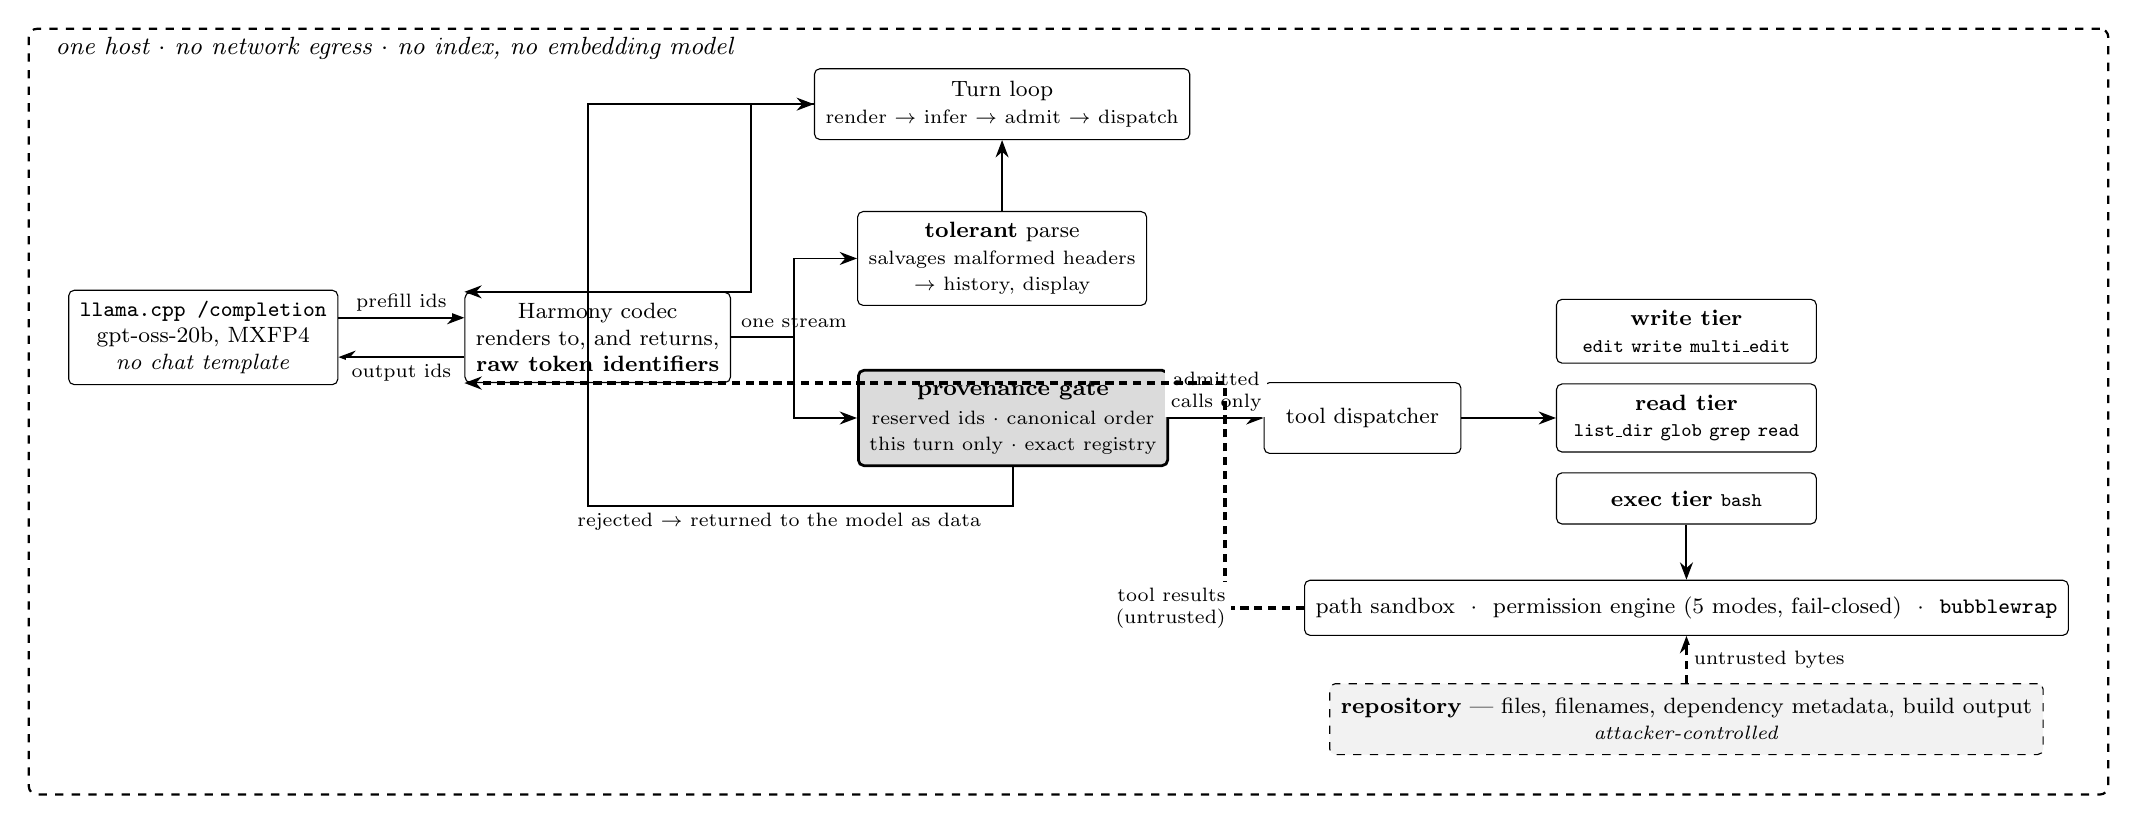
\begin{tikzpicture}[
  font=\footnotesize,
  blk/.style       = {draw, rounded corners=2pt, align=center, inner sep=4pt,
                      minimum height=9mm, minimum width=27mm, fill=white},
  gate/.style      = {blk, fill=black!14, line width=1pt, minimum width=34mm},
  tier/.style      = {blk, minimum width=33mm, minimum height=6.5mm},
  untrusted/.style = {blk, dashed, fill=black!5},
  ar/.style        = {-{Stealth[length=2.2mm]}, line width=0.7pt},
  arth/.style      = {-{Stealth[length=2.2mm]}, line width=1.4pt, densely dashed},
  lbl/.style       = {font=\scriptsize, inner sep=2pt, fill=white}
]

% ---- model path -----------------------------------------------------------
\node[blk, minimum width=30mm] (srv)
  {\texttt{llama.cpp /completion}\\gpt-oss-20b, MXFP4\\\emph{no chat template}};

\node[blk, right=16mm of srv, minimum width=30mm] (codec)
  {Harmony codec\\renders to, and returns,\\\textbf{raw token identifiers}};

\draw[ar] ([yshift=2.5mm]srv.east) -- node[lbl, above]{prefill ids}
          ([yshift=2.5mm]codec.west);
\draw[ar] ([yshift=-2.5mm]codec.west) -- node[lbl, below]{output ids}
          ([yshift=-2.5mm]srv.east);

% ---- the fork: one token stream, two consumers ----------------------------
\coordinate (fork) at ($(codec.east)+(8mm,0)$);
\draw[line width=0.7pt] (codec.east) -- (fork);
\node[lbl, above=0.5mm of fork] {one stream};

\node[blk, above right=4mm and 8mm of fork, minimum width=36mm] (parse)
  {\textbf{tolerant} parse\\\scriptsize salvages malformed headers\\
   \scriptsize $\rightarrow$ history, display};

\node[gate, below right=4mm and 8mm of fork] (gate)
  {\textbf{provenance gate}\\[1pt]
   \scriptsize reserved ids $\cdot$ canonical order\\
   \scriptsize this turn only $\cdot$ exact registry};

\draw[ar] (fork) |- (parse.west);
\draw[ar] (fork) |- (gate.west);

\node[blk, right=12mm of gate, minimum width=25mm] (disp) {tool dispatcher};
\draw[ar] (gate) -- node[lbl, above, align=center]{admitted\\calls only} (disp);

% ---- turn loop, and the rejection path ------------------------------------
\node[blk, above=9mm of parse, minimum width=40mm] (loop)
  {Turn loop\\\scriptsize render $\rightarrow$ infer $\rightarrow$ admit $\rightarrow$ dispatch};
\draw[ar] (parse) -- (loop);
\draw[ar] (loop.west) -- ++(-8mm,0) |- (codec.north west);

\draw[ar] (gate.south) -- ++(0,-5mm) -- ++(-54mm,0)
  node[lbl, pos=0.55, below, align=center]{rejected $\rightarrow$ returned to the model as data}
  |- (loop.west);

% ---- tool tiers -----------------------------------------------------------
\node[tier, right=12mm of disp] (read)
  {\textbf{read tier}\\\scriptsize \texttt{list\_dir} \texttt{glob} \texttt{grep} \texttt{read}};
\node[tier, below=2.5mm of read] (exec)
  {\textbf{exec tier} \scriptsize \texttt{bash}};
\node[tier, above=2.5mm of read] (write)
  {\textbf{write tier}\\\scriptsize \texttt{edit} \texttt{write} \texttt{multi\_edit}};
\draw[ar] (disp) -- (read);

% ---- enforcement and the untrusted source ---------------------------------
\node[blk, below=7mm of exec, minimum width=70mm, minimum height=7mm] (enf)
  {path sandbox \ $\cdot$ \ permission engine (5 modes, fail-closed)
   \ $\cdot$ \ \texttt{bubblewrap}};
\draw[ar] (exec) -- (enf);

\node[untrusted, below=6mm of enf, minimum width=70mm] (repo)
  {\textbf{repository} --- files, filenames, dependency metadata, build output\\
   \scriptsize \emph{attacker-controlled}};
\draw[arth] (repo) -- node[lbl, right]{untrusted bytes} (enf);

% ---- the edge that closes the loop, and why the gate is upstream of it ----
\draw[arth] (enf.west) -- ++(-10mm,0)
  node[lbl, pos=0.9, left, align=right]{tool results\\(untrusted)}
  |- (codec.south west);

% ---- host boundary --------------------------------------------------------
\node[draw, dashed, line width=0.8pt, rounded corners=3pt,
      fit=(srv)(loop)(write)(repo)(enf)(gate), inner sep=5mm] (host) {};
\node[anchor=north west, font=\small\itshape] at (host.north west)
  {\ \ one host $\cdot$ no network egress $\cdot$ no index, no embedding model};

\end{tikzpicture}%
}

\caption{The offline code agent used in this work. The Harmony prompt is
rendered to raw token identifiers client-side and the returned identifiers are
parsed client-side, so no chat template intervenes: this is what makes the
admission policy explicit at the call site and a token-level provenance check
possible at all. One token stream has two consumers, and deliberately not one
implementation. The tolerant parser feeds history and display, salvaging
malformed headers so a bad completion does not waste a turn; the provenance gate
feeds dispatch, and refuses them. A text-level check cannot occupy the lower
path, because the distinction it would have to make is absent from decoded text.
Dashed nodes are attacker-controlled; the shaded node is contributed here.}
\label{fig:system}
\end{figure*}

\subsection{The Harmony response format}

Harmony gives every message a role and a channel, delimited by reserved
tokens~\cite{openai2025gptoss,harmony2026}. An assistant turn may carry private
reasoning on the \texttt{analysis} channel, tool calls on \texttt{commentary},
and the user-facing answer on \texttt{final}. A tool call has the form

\begin{center}\small
\hmtok{channel}\texttt{commentary to=functions.read}\\
\hmtok{constrain}\texttt{json}\hmtok{message}\texttt{\{...\}}\hmtok{call}
\end{center}

\noindent
The reserved tokens are \hmtok{start}, \hmtok{end}, \hmtok{message},
\hmtok{channel}, \hmtok{constrain}, \hmtok{call}, and \hmtok{return}.

\subsection{The agent}

Fig.~\ref{fig:system} shows the system: a single-agent reason--act--observe
loop~\cite{yao2023react} with no agent framework. Using the reference
renderer~\cite{openaiharmony}, it renders the conversation directly to token
identifiers and parses returned identifiers back into channels, driving the
server's raw completion endpoint rather than a chat-completions abstraction.
Two consequences matter. The agent, not the server, chooses the admission policy
for special tokens, so the variable this paper measures is explicit in its
source. And the orchestrator holds the identifiers themselves, so it can check
their provenance, which a client speaking through a chat-completions
abstraction cannot.

Tools form a navigation funnel (\texttt{list\_dir}, \texttt{glob},
\texttt{grep}, \texttt{read}) with an opt-in execution tier and a
permission-gated write tier. A path sandbox confines file access, a five-mode
permission engine resolves each mutating call and fails closed, and
\texttt{bubblewrap} confines execution where available. One limitation is stated
rather than concealed: the inference client reaches the model server over
unauthenticated HTTP, which is sound on loopback and not across a network.

\subsection{Threat model}
\label{sec:threat}

The developer and the shell they already possess are trusted. Repository file
contents, filenames, dependency metadata, and command output are untrusted: an
attacker who can contribute to a project controls them. A malicious model, a
compromised inference server, and hardware attacks are out of scope. The
attacker's goal is to cause the orchestrator to execute a tool invocation the
developer did not request, by placing bytes where the agent will read them. This
is the standard indirect setting~\cite{greshake2023indirect,zhan2024injecagent,
debenedetti2024agentdojo}.

% ==========================================================================
\section{Exposure Is Renderer-Determined}
\label{sec:renderer}
% ==========================================================================

\subsection{Where the admission decision is made}

Let $u$ be a byte string under attacker control that contains the characters of
a Harmony control token, and let $R$ be a renderer that assembles a prompt from
a conversation containing $u$. The security-relevant question is not what $u$
decodes to --- that is fixed --- but whether $R$ emits the reserved identifier
for that marker, or a sequence of ordinary subword identifiers with the same
decoding.

For a Hugging Face chat template, this is governed by whether the tokenizer
configuration declares the marker special, which is the variable Zhan et al.
audit. For Harmony it is governed by an argument at the call site: the reference
renderer exposes an explicit allowed- and disallowed-special policy, so the same
library yields different answers depending on how it is invoked. A configuration
audit is therefore not merely incomplete for this format; it measures the wrong
object, and reports absence where a per-call-site measurement is required.

\subsection{The rendering paths a Harmony agent can take}

We enumerate the paths an integrator realistically takes and treat each as an
experimental arm: the reference renderer's conversation-rendering entry point;
its direct encoding entry point under the default policy; the same under a
permissive policy; and server-side templating, where the serving stack applies
Harmony and the client never sees identifiers. The harness measured
by~\cite{usama2026controltoken} is included as a fifth arm and as the source of
the reference attack. Table~\ref{tab:renderer} reports the outcome.

\subsection{Why this is not a configuration defect}

Nothing here is a bug in any one component. Each path is a reasonable reading of
its own interface, and an integrator choosing between them is not warned that
the choice is a security decision. That is the point of C1: the variable that
decides whether the attack of~\cite{usama2026controltoken} works is a function
argument, and no published audit records it.

That the paths genuinely diverge in deployment is visible independently of our
measurements. A source-code study of eleven coding agents finds the layer to be
hand-rolled in each~\cite{harness2026}; one serving stack has been reported to
return a malformed Harmony header as a tool call whose name matches no
registered tool~\cite{vllmharmony}; malformed Harmony headers are reported in
roughly four per cent of turns at temperature 1.0~\cite{llamacppharmony}; and
gpt-oss has been observed emitting Harmony special markers as ordinary subwords
under long prompts~\cite{unslothharmony} --- the same admission question arising
from the model's side rather than the renderer's. We cite these as evidence that
the behaviour varies in practice, not as results.

% ==========================================================================
\section{Textual Control Fields}
\label{sec:recipient}
% ==========================================================================

\begin{figure}[t]
\centering
% ---------------------------------------------------------------------------
% Fig. 2 -- Anatomy of a Harmony tool-call header: a control plane that is
% part reserved token, part plain text.
%
% This is the conceptual core of the paper. The point the figure must make:
% the three shaded-dashed cells carry control meaning but have no reserved
% token identity, so no tokenizer-level defense can protect them -- and one of
% them, the recipient, selects which tool executes.
%
% Single column. \hmtok{} is defined in main.tex.
% ---------------------------------------------------------------------------
\resizebox{\columnwidth}{!}{%
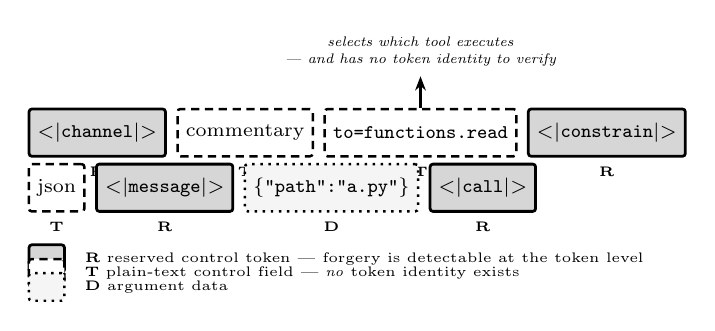
\begin{tikzpicture}[
  font=\scriptsize,
  res/.style = {draw, line width=1pt, fill=black!16, rounded corners=1pt,
                align=center, inner sep=3pt, minimum height=6mm},
  txt/.style = {draw, densely dashed, line width=0.9pt, fill=white,
                rounded corners=1pt, align=center, inner sep=3pt,
                minimum height=6mm},
  dat/.style = {draw, dotted, line width=0.9pt, fill=black!4,
                rounded corners=1pt, align=center, inner sep=3pt,
                minimum height=6mm},
  cls/.style = {font=\tiny\bfseries, inner sep=1pt}
]

% ---------- line 1 ---------------------------------------------------------
\node[res] (a1) {\hmtok{channel}};
\node[txt, right=1.2mm of a1] (a2) {commentary};
\node[txt, right=1.2mm of a2] (a3) {\texttt{to=functions.read}};
\node[res, right=1.2mm of a3] (a4) {\hmtok{constrain}};

\node[cls, below=0.8mm of a1] {R};
\node[cls, below=0.8mm of a2] {T};
\node[cls, below=0.8mm of a3] {T};
\node[cls, below=0.8mm of a4] {R};

% ---------- line 2 ---------------------------------------------------------
\node[txt, below=7mm of a1.west, anchor=west] (b1) {json};
\node[res, right=1.2mm of b1] (b2) {\hmtok{message}};
\node[dat, right=1.2mm of b2] (b3) {\texttt{\{"path":"a.py"\}}};
\node[res, right=1.2mm of b3] (b4) {\hmtok{call}};

\node[cls, below=0.8mm of b1] {T};
\node[cls, below=0.8mm of b2] {R};
\node[cls, below=0.8mm of b3] {D};
\node[cls, below=0.8mm of b4] {R};

% ---------- the field that decides which tool runs -------------------------
\draw[-{Stealth[length=1.8mm]}, line width=0.9pt]
  (a3.north) -- ++(0,4mm)
  node[above, font=\tiny\itshape, align=center]
  {selects which tool executes\\--- and has no token identity to verify};

% ---------- legend ---------------------------------------------------------
\node[res, below=9mm of b1.west, anchor=west,
      minimum width=4.5mm, minimum height=3.5mm, inner sep=0pt] (lr) {};
\node[anchor=west, right=1.2mm of lr, font=\tiny, align=left]
  {\textbf{R} reserved control token --- forgery is detectable at the token
   level};

\node[txt, below=1.8mm of lr.west, anchor=west,
      minimum width=4.5mm, minimum height=3.5mm, inner sep=0pt] (lt) {};
\node[anchor=west, right=1.2mm of lt, font=\tiny, align=left]
  {\textbf{T} plain-text control field --- \emph{no} token identity exists};

\node[dat, below=1.8mm of lt.west, anchor=west,
      minimum width=4.5mm, minimum height=3.5mm, inner sep=0pt] (ld) {};
\node[anchor=west, right=1.2mm of ld, font=\tiny, align=left]
  {\textbf{D} argument data};

\end{tikzpicture}%
}

\caption{A Harmony tool-call header interleaves two classes of control field.
Cells marked \textbf{R} are reserved control tokens: a forgery is detectable,
because the genuine field is one identifier and the forgery is a sequence of
subword identifiers decoding to the same bytes. Cells marked \textbf{T} carry
control meaning but are ordinary text, so there is no identity to check and no
tokenizer-level defense applies. The recipient is class \textbf{T}, and it
selects the tool that executes.}
\label{fig:controlplane}
\end{figure}

\subsection{Two classes, and why only one is defensible}

Partition the regions an orchestrator consults when deciding whether and how to
dispatch a call.

\textbf{Class R, reserved control fields.} Realised as a single reserved
identifier. A forgery built from untrusted text is distinguishable from a
genuine field, because the two differ in identifiers while agreeing in bytes.
This is the distinction whose behavioural consequence~\cite{zhan2026samebytes}
measures and which~\cite{yang2026nameless} defends by removing surface strings
from control tokens while preserving their identifiers.

\textbf{Class T, textual control fields.} Realised as ordinary text, yet
consulted for control. A forgery is \emph{indistinguishable} from a genuine
field at every level available to the orchestrator, because the genuine field is
also ordinary text. Renaming reserved tokens does not help: there is no reserved
token.

Table~\ref{tab:fields} gives the partition for Harmony. Four fields are class R
and three are class T. This is a property of the format, established by
inspection, and is the only claim in this paper that is not measured.

\subsection{The recipient}

Of the three class-T fields, the recipient \texttt{to=functions.$\langle$tool
$\rangle$} is consequential, because it is the field from which the orchestrator
reads the name of the tool to execute. An orchestrator that recovers a recipient
from text is making an execution decision on evidence it cannot authenticate.

This field is unexamined in the literature. In~\cite{usama2026controltoken} the
string \texttt{to=functions} appears only inside verbatim generation listings,
and the recipient is never treated as an attack surface; the paper's parser
contribution concerns one property, whether the pattern tolerates a missing
closing \hmtok{call}, and its hardening recommendation is to require that
token. In~\cite{zhan2026samebytes} Harmony does not appear. Recent surveys of
agentic security do not reach this layer at all: a 2026 survey of threats,
defenses, evaluation and open challenges names long-horizon behaviour,
multi-agent settings, benchmarks, adaptive attacks, and embodied agents as the
open problems, and does not list the harness~\cite{chhabra2026agentic}; a
contemporaneous review characterises delimiter-based isolation as failing
because natural language can persuade a model to ignore
delimiters~\cite{gulyamov2026promptinj}, whereas the mechanism
of~\cite{zhan2026samebytes} is representational rather than rhetorical; and a
systematisation of prompt injection against coding assistants, covering 78
studies and 42 techniques, reports that adaptive attacks exceed 85\% success and
that most of 18 surveyed defenses mitigate under 50\%, without considering
tokenization~\cite{maloyan2026coding}.

% ==========================================================================
\section{The Control-Token Provenance Gate}
\label{sec:defense}
% ==========================================================================

\begin{figure}[t]
\centering
% ---------------------------------------------------------------------------
% Fig. 3 -- The path from attacker-controlled bytes to tool execution, and the
% point at which the provenance gate severs it.
%
% Greyscale-safe: no colour carries meaning. The cut is drawn, not symbolic,
% so it survives black-and-white printing.
%
% Single column.
% ---------------------------------------------------------------------------
\resizebox{\columnwidth}{!}{%
\begin{tikzpicture}[
  font=\scriptsize,
  step/.style  = {draw, rounded corners=2pt, align=center, inner sep=3.5pt,
                  minimum height=6.5mm, text width=52mm, fill=white},
  untr/.style  = {step, densely dashed, fill=black!6},
  gate/.style  = {step, fill=black!14, line width=1pt},
  sink/.style  = {step, fill=white},
  ar/.style    = {-{Stealth[length=2mm]}, line width=0.7pt},
  num/.style   = {font=\tiny\bfseries, inner sep=1pt}
]

\node[untr] (s1)
  {\textbf{1} \ A repository file contains a header-shaped span\\
   \scriptsize\texttt{...\hmtok{channel}commentary to=functions.bash...}};

\node[untr, below=3.2mm of s1] (s2)
  {\textbf{2} \ \texttt{read} or \texttt{grep} returns it as a tool result};

\node[step, below=3.2mm of s2] (s3)
  {\textbf{3} \ The result enters the context verbatim};

\node[step, below=3.2mm of s3] (s4)
  {\textbf{4} \ The model restates it while reasoning\\
   \scriptsize(ordinary behaviour when summarising a file)};

\node[step, below=3.2mm of s4] (s5)
  {\textbf{5} \ A header-shaped span appears in model output ---\\
   \scriptsize \emph{byte-identical} to a header the model authored};

\node[gate, below=4.5mm of s5] (g)
  {\textbf{Control-token provenance gate}\\
   \scriptsize reserved-ID sequence must be canonical\\
   \scriptsize recipient must match the registry exactly};

\node[sink, below=7mm of g] (s7)
  {\textbf{6} \ \texttt{bash} executes the attacker's command};

\draw[ar] (s1) -- (s2);
\draw[ar] (s2) -- (s3);
\draw[ar] (s3) -- (s4);
\draw[ar] (s4) -- (s5);
\draw[ar] (s5) -- (g);
\draw[ar] (g)  -- (s7);

% ---- the cut --------------------------------------------------------------
\coordinate (cut) at ($(g.south)!0.5!(s7.north)$);
\draw[line width=1.1pt] ($(cut)+(-2mm,-2mm)$) -- ($(cut)+(2mm,2mm)$);
\draw[line width=1.1pt] ($(cut)+(-2mm,2mm)$) -- ($(cut)+(2mm,-2mm)$);
\node[anchor=west, font=\tiny\itshape, align=left] at ($(cut)+(4mm,0)$)
  {no reserved-ID header\\$\Rightarrow$ not a call};

% ---- what the gate replaces ----------------------------------------------
\node[anchor=east, font=\tiny\itshape, align=right, text width=22mm]
  at ($(g.west)+(-2mm,0)$)
  {replaces tolerant parsing and prose-level recovery};

\end{tikzpicture}%
}

\caption{From attacker-controlled bytes to tool execution, and the two
independent points at which the path can be cut. Steps 1--5 are ordinary agent
behaviour rather than an exploit: an agent that reads a file restates it. The
renderer decides whether the forged span ever acquires reserved identifiers
(C1); the gate decides whether a span lacking them can become a call (C3).
Either cut alone breaks the chain, which is why the security claim does not rest
on one of them. The categories on the right are what the gate reports in place
of a repaired call, and they are the measurement grain of
Table~\ref{tab:gate}.}
\label{fig:dispatch}
\end{figure}

\subsection{Specification}

The gate sits between parsing and dispatch (Fig.~\ref{fig:system}) and admits a
candidate call only if all four conditions hold.

\begin{enumerate}
\item \textbf{Reserved-identifier provenance.} Every class-R field of the
candidate's header is present in the completion as that marker's reserved
identifier, not as any other sequence decoding to the same bytes.
\item \textbf{Canonical ordering.} Those identifiers occur in the order the
format specifies for a tool call, with no interleaved reserved token and no
repetition.
\item \textbf{Turn provenance.} The candidate is drawn from the identifiers
returned by the current turn's inference request, not from text that entered the
context as a tool result or as history.
\item \textbf{Registry exactness.} After the canonical header prefix, the
recipient equals the name of a registered tool by exact string comparison. No
prefix, suffix, case, or edit-distance matching.
\end{enumerate}

A failing candidate is not dispatched; it returns to the model as data, so a
genuine malformation costs a turn rather than crashing the agent, and no
fallback reconstructs a call from prose. The gate reports which condition
failed, in the nine categories of Fig.~\ref{fig:dispatch}, so a rejection is a
measurement rather than a silent drop.

\textbf{Implementation.} The gate is about 230 lines of Python operating on the
identifier sequence returned by one completion, with 31 unit tests. It does
not reuse the agent's existing parser: that parser is deliberately tolerant,
because salvaging a malformed header keeps a transcript renderable and avoids
wasting a turn, and tolerance is exactly the wrong property for deciding what to
execute. The two consumers of the token stream are therefore separate code
paths (Fig.~\ref{fig:system}), which is a design consequence of the argument in
this paper rather than an implementation detail.

\subsection{Why a gate and not a sanitiser}

Conditions 1 to 3 restore to class-R fields the authentication that client-side
rendering makes available. Condition 4 is what class T admits instead:
unverifiable, so confined to a closed set the orchestrator already trusts.

The alternative in the literature is to neutralise control tokens in untrusted
input before templating. Usama et al. evaluate exactly this and report both that
it works and how it fails: deleting control-token spans splices the residual
role and channel words into \texttt{assistantanalysis}, which is itself
sufficient to suppress the reasoning channel, so sanitisation must replace or
escape rather than delete~\cite{usama2026controltoken}. That is a string-level
contest over which spans to rewrite. The gate does not enter it. It does not
inspect untrusted text for dangerous substrings; it declines to derive control
structure from anything but identifiers whose provenance it can establish, which
leaves the attacker no spelling to adjust.

The gate also generalises their parser hardening. Requiring the closing
\hmtok{call} is condition~2 restricted to one token; conditions 1 to 4 extend
the same reasoning to the whole header, including the recipient their
recommendation does not cover.

\subsection{Scope and cost}

The gate does not detect malicious intent, inspect argument values, or reason
about command semantics; those belong to the authorization layer above it, which
operates on parsed structured calls~\cite{zhang2026agate,lingering2026}. It
performs integer comparisons over identifiers the orchestrator already holds,
issues no additional inference request, and imposes no decoding constraint, so
it cannot incur the reasoning or tool-invocation costs reported for
schema-constrained decoding~\cite{constrainttax2026,structfail2026}. Its cost is
the utility lost when a genuine but malformed call is refused rather than
repaired, reported directly in Section~\ref{sec:results}.

% ==========================================================================
\section{Evaluation Design}
\label{sec:eval}
% ==========================================================================

\textbf{Platform.} gpt-oss-20b in native MXFP4, served by a single-slot local
server on one \PH{GPU model, VRAM} with a \PH{ctx}-token context. Sampling is
fixed and reported; dependencies are pinned by exact version, including the
renderer, whose version determines the prompt bytes.

\textbf{Determinism.} One greedy reference run per configuration, whose bitwise
reproducibility on a single slot we verify rather than assume, plus reliability
over $k=\PH{k}$ independent sampled draws. We state whether per-request seeding
of sampled decoding is honoured by the build, because a mean over sampled runs
is not reproducible if it is not.

\textbf{Reference attack.} The published suffix
of~\cite{usama2026controltoken}, whose code and per-trial logs are available, is
run against every arm. This is a replication and is reported as such.

\textbf{Forgery corpus.} \PH{N} cases, the cross product of \PH{M} target fields
(seven reserved markers and three textual control fields) with \PH{K} untrusted
channels --- file contents, filenames, dependency metadata, command output ---
and \PH{P} payload classes. Each case carries a machine-checkable oracle naming
the action that must not occur.

\textbf{Measured quantities.} The \emph{admission outcome} is whether a forged
field acquires its reserved identifier in the rendered prompt, read directly off
the identifier sequence with no inference. The \emph{dispatch outcome} is
whether the agent executed the forged call, decided by the oracle.

\textbf{Arms.} Renderer (the paths of Section~\ref{sec:renderer}) $\times$
orchestrator $\in$ \{strict parse, tolerant parse, tolerant parse with
prose-level recovery, provenance gate\}.

\textbf{Utility.} To price the gate we report task success on \PH{Q} repository
questions over \PH{R} open-source repositories, each annotated with the file and
line ranges that must be consulted, which makes grounding checkable without a
judge. A judge is unavailable by construction here: a hosted one contradicts the
offline premise, and the model under test is circular.

% ==========================================================================
\section{Results}
\label{sec:results}
% ==========================================================================

\begin{table}[t]
\caption{Control-field classification for a Harmony tool-call header.
Token counts are measured against the released vocabulary; a field is
defensible at the token level only if it is a single \emph{reserved}
identifier.}
\label{tab:fields}
\centering
\small
\begin{tabular}{@{}llcc@{}}
\toprule
\textbf{Field} & \textbf{Class} & \textbf{Tokens} & \textbf{Forgery detectable?} \\
\midrule
\hmtok{channel}            & R & 1 & yes \\
\texttt{commentary}        & T & 2 & \textbf{no} \\
\texttt{to=functions.read} & T & 4 & \textbf{no} \\
\hmtok{constrain}          & R & 1 & yes \\
\texttt{json}              & T & 1 & \textbf{no} \\
\hmtok{message}            & R & 1 & yes \\
\hmtok{call}               & R & 1 & yes \\
\bottomrule
\end{tabular}
\end{table}

\begin{table}[t]
\caption{C1: the same bytes under each rendering path. The admission column is
decided by the renderer and the vocabulary alone and requires no inference; the
behavioural columns are reliability@$k$ over the task suite. The final row is
the measurement published by~\cite{usama2026controltoken}, whose rendering path
is a Hugging Face chat template.}
\label{tab:renderer}
\centering
\small
\begin{tabular}{@{}lccc@{}}
\toprule
\textbf{Rendering path} & \textbf{Reserved ids} & \textbf{Ref.\ attack} & \textbf{Dispatch} \\
                        & \textbf{admitted}     & \textbf{succ.\ \%}    & \textbf{rate \%}  \\
\midrule
Reference renderer, tool result  & 0 of 7  & \PH{..} & \PH{..} \\
Reference renderer, user message & 0 of 7  & \PH{..} & \PH{..} \\
Reference renderer, default      & refused & \PH{..} & \PH{..} \\
Reference renderer, permissive   & 5 of 7  & \PH{..} & \PH{..} \\
Server-side templating           & \PH{..} & \PH{..} & \PH{..} \\
Chat template~\cite{usama2026controltoken} & 5 of 7 & 100 & 100 \\
\bottomrule
\end{tabular}
\end{table}

\begin{table}[t]
\caption{C3: forged-call dispatch and utility by orchestrator}
\label{tab:gate}
\centering
\small
\begin{tabular}{@{}lccc@{}}
\toprule
\textbf{Orchestrator} & \textbf{Dispatch} & \textbf{Task} & \textbf{Turns} \\
                      & \textbf{rate \%}  & \textbf{succ.\ \%} & \textbf{/task} \\
\midrule
Strict parse                 & \PH{..} & \PH{..} & \PH{..} \\
\quad + tolerant parse       & \PH{..} & \PH{..} & \PH{..} \\
\quad + prose-level recovery & \PH{..} & \PH{..} & \PH{..} \\
Input sanitisation~\cite{usama2026controltoken} & \PH{..} & \PH{..} & \PH{..} \\
\textbf{Provenance gate (ours)} & \PH{..} & \PH{..} & \PH{..} \\
\bottomrule
\end{tabular}
\end{table}

\subsection{Admission is renderer-determined}

Table~\ref{tab:renderer} reports the C1 result for the published reference
payload, with model, bytes and decode held fixed and the rendering path as the
only variable. Under the reference renderer's conversation-rendering entry
point, none of the seven forged markers acquires a reserved identifier,
whether the payload arrives in a tool result or in the user turn; the direct
encoding entry point refuses the payload outright under its default policy; and
under a permissive policy five of seven acquire reserved identifiers. The same
five acquire reserved identifiers under the Hugging Face chat template used
by~\cite{usama2026controltoken}, which is how we calibrate: our permissive arm
reproduces their published token sequence exactly, so the measurement
instrument agrees with theirs where the paths agree and diverges only where the
paths diverge.

Two observations follow. The attack of~\cite{usama2026controltoken} is not
blocked here by any defense; it is blocked by an argument default. And nothing
in the audit of~\cite{zhan2026samebytes} could have recorded this, because the
Harmony control tokens are not registered as declared-special: their own
released measurement notes that these are \emph{``single dedicated
reserved-vocabulary tokens\,\ldots\ that are not in that
registry''}~\cite{usama2026controltoken}, which is precisely why a
declared-special audit reports zero for gpt-oss while the tokenizer still emits
those identifiers from untrusted text.

\subsection{The recipient is not a token}

Table~\ref{tab:fields} reports the classification of
Section~\ref{sec:recipient}, measured against the released vocabulary. Four of
the seven control fields are a single reserved identifier. Three are not:
\texttt{commentary} is two tokens, \texttt{to=functions.read} is four, and
\texttt{json}, although one token, is an ordinary one. A forgery of any of the
three is indistinguishable from the genuine field, and the four-token case is
the recipient. The same tokenisation is visible in the generations published
by~\cite{usama2026controltoken}, where \texttt{commentary} appears as two
ordinary tokens and the recipient as five, so this is a property of the
vocabulary rather than of our rendering path.

\subsection{Cost of the gate}

Table~\ref{tab:gate} prices the gate against the orchestrator configurations it
replaces, including the input sanitisation of~\cite{usama2026controltoken} as
the published alternative.

The behavioural measurements are in progress and those cells are unpopulated.
We commit in advance to reporting the following should they occur: that the
reference attack succeeds under the path this agent uses, which would refute
C1; that the gate costs more task success than prose-level recovery gains; and
any case in which a class-T forgery is dispatched despite the gate.

% ==========================================================================
\section{Related Work}
% ==========================================================================

\textbf{Control tokens on Harmony.} The closest work
is~\cite{usama2026controltoken}, which measures control-token injection on
gpt-oss-20b under Harmony, establishes that the harness rather than the model
decides whether a call fires, and evaluates sanitisation, parser hardening, and
empty-reasoning detection as defenses. We take its result as established and
differ in three respects: it varies the chat template across models, while we
vary the renderer within one format and show that this is what reconciles it
with~\cite{zhan2026samebytes}; it addresses the reasoning channel, while we
address the field that names the tool; and its defense rewrites untrusted input,
while ours conditions dispatch on provenance.

\textbf{The reserved-identifier mechanism.} Zhan et
al.~\cite{zhan2026samebytes} separate a forged marker's text from its token
identity and localise the attack's authority to the learned vector at the marker
position. Their audit of tokenizer configurations is the methodology we argue
cannot describe Harmony. Yang et al.~\cite{yang2026nameless} defend at the
tokenizer by removing surface strings from control tokens; the two defenses
compose, and neither reaches a class-T field.

\textbf{Chat-template injection.} Forging template structure to elevate an
injected instruction originates with ChatInject~\cite{chang2026chatinject} and
has since been automated~\cite{deng2026structural}; related attacks manipulate
special tokens directly~\cite{metabreak2025,badtemplate2026}. Security probes of
gpt-oss-20b report guardrail bypasses under adversarial
framing~\cite{durner2025harmony}. These works forge structure in order to
execute an instruction; we ask who is entitled to author the structure at all.

\textbf{Agent authorization.} AGATE gates invocation on authorization and data
provenance at an instrumented dispatch boundary~\cite{zhang2026agate}; related
work bounds agents by execution provenance~\cite{agentsentry2026} or revocable
capabilities~\cite{lingering2026}. These reason about parsed structured calls
and presuppose what our gate establishes: that the call corresponds to control
tokens the model actually emitted.

\textbf{Indirect prompt injection.} The setting is
established in~\cite{greshake2023indirect} and benchmarked
in~\cite{zhan2024injecagent,debenedetti2024agentdojo} and, in increasingly
realistic deployments, in~\cite{livepi2026,netinject2026,issuetrojan2026};
surface-level defenses are defeated adaptively~\cite{framinggap2026}, and
open-weight models are broadly exposed to prefill
attacks~\cite{prefill2026}. Execution security for coding agents, including
isolation and time-of-check-to-time-of-use weaknesses, is surveyed
in~\cite{balkan2026}.

\textbf{Structured generation.} Grammar- and schema-constrained
decoding~\cite{willard2023outlines} makes malformed output impossible rather
than recoverable, at a reported cost in reasoning quality and in tool invocation
itself~\cite{constrainttax2026,structfail2026}; constraining only the structured
region reduces that cost~\cite{crane2025,inwriting2026}. Our gate is not a
decoding method: it adds no constraint and no inference, and verifies provenance
after generation rather than shaping it.

% ==========================================================================
\section{Threats to Validity}
\label{sec:validity}
% ==========================================================================

\textbf{Construct.} The admission outcome records whether a forged field
acquired a reserved identifier. It does not establish behavioural consequence,
which is why the dispatch outcome is measured separately rather than inferred.

\textbf{Internal.} Numerical non-determinism in batched inference is a known
confound. We use a single server slot and verify bitwise reproducibility of the
greedy reference run. Where per-request seeding of sampled decoding is not
honoured, reliability is computed from independent draws and an individual
sampled run is not reproducible; we state which case applies.

\textbf{External.} One model of one family, \PH{R} repositories, and one
response format. The class-R/class-T partition requires a format that
interleaves reserved tokens with textual control fields; we expect this to
generalise but do not demonstrate it.

\textbf{Conclusion.} The security result rests on a corpus we constructed, which
cannot be exhaustive, and on one replication of a published attack. It
establishes a lower bound on exposure, not an upper bound on safety.

\textbf{Ethics.} All attacks were constructed against a fixture repository and an
agent operated by the authors, on an isolated host with no network egress. No
third-party system was targeted. The reference attack is already public.

% ==========================================================================
\section{Conclusion}
\label{sec:conclusion}
% ==========================================================================

Whether a Harmony agent is exposed to control-token forgery is decided by the
renderer, not by the tokenizer configuration the literature audits, which is why
one study can break gpt-oss through a forged tool-protocol structure while
another, days later, records it as having none. Auditing the renderer is
necessary but not sufficient: part of Harmony's control plane is not a token, and
the part that selects which tool executes is exactly that part. We therefore
condition dispatch on provenance rather than rewriting untrusted input --- a call
is admitted only on canonical reserved identifiers from the admitted turn plus
exact registry equality --- which costs integer comparisons, no inference, and
leaves no spelling for an attacker to adjust.

Future work extends the check into generation, so that the orchestrator emits
the canonical header itself and a forged one is unreachable rather than merely
inadmissible, and characterises textual control fields in formats beyond
Harmony.

\PH{Artifact availability statement --- remove if review is double-blind.}

\section*{Acknowledgment}

\PH{Acknowledgements, compute provider, and funding, if any.}

\bibliographystyle{IEEEtran}
\bibliography{references}

\end{document}
